\documentclass[10pt]{beamer}
\usetheme{metropolis}
\usecolortheme{spruce}
\setbeamercolor{structure}{fg=lmugreen}
\usepackage[english]{babel}
\usepackage{tipa}
\usepackage[utf8]{inputenc}
\usepackage{graphicx}
\usepackage[abs]{overpic}
\usepackage{tikz}
\usepackage{mwe}
\usepackage{amsmath,amssymb,amsfonts,amsthm}
\usepackage{mathtools}
\usepackage{listings}
\usepackage[ruled,vlined]{algorithm2e}
\usepackage{hyperref}
\usepackage{textcomp}
\usepackage{braket}
\usepackage{csquotes}
\usepackage{tikz}
\usepackage{calc}
\usepackage{tcolorbox}

\usepackage[style=chem-angew,backend=biber]{biblatex}
\addbibresource{literatur.bib}

% \hypersetup{colorlinks,breaklinks,
% urlcolor=black,
% linkcolor=black,
% citecolor=black,
% }
\usepackage[export]{adjustbox}
\usepackage{float}
% 表格
\usepackage{tabularx}
\setbeamerfont{caption}{size=\scriptsize}
% 动画
\usepackage{animate}
% 背景

\usepackage{tikz}
\usetikzlibrary{arrows,shapes}
\tikzstyle{block} = [rectangle, draw, fill=blue!20,
text width=10em, text centered, rounded corners, node distance=1cm, minimum height=2em]
\tikzstyle{line} = [draw, -latex']

\usebackgroundtemplate
{
% \begin{picture}(200,200)
% \put(243,-85)
% {\hbox{
% \begin{tikzpicture}
%     \node[opacity=0.1]{\includegraphics[width=5cm]{bilder/lmulogo}};%
% \end{tikzpicture}
% }}
% \end{picture}
}
\definecolor{lmugreen}{RGB}{0,102,51}

\title[Adaptive Biasing Methods]{
    Calculation of Free Energy Curves along Reaction Coordinates with Adaptive Biasing Methods
}
\author[Andreas Hulm, 2021]{
    Andreas Hulm
}
\institute[LMU]{
    LMU Munich \\
  %  \texttt{\href{firstname.lastname@campus.lmu.de}{firstname.lastname@campus.lmu.de}}
    }
\date[Masterthesis, \today]{
    Master Thesis, Munich, Germany\\
    \today
}

% % Definition Progressbar
\makeatletter
\newlength{\custom@progressinheadfoot}
\setbeamertemplate{progress bar in head/foot}{
    \nointerlineskip
    \setlength{\custom@progressinheadfoot}{%
        \paperwidth * \ratio{\insertframenumber pt}{\inserttotalframenumber pt}%
    }%
    \begin{beamercolorbox}[wd=\paperwidth]{progress bar in head/foot}
        \begin{tikzpicture}
            \draw[bg, fill=bg] (0,0) rectangle (\paperwidth, 0.17em);
            \draw[fg, fill=fg] (0,0) rectangle (\custom@progressinheadfoot, 0.17em);
        \end{tikzpicture}%
    \end{beamercolorbox}
}
\addtobeamertemplate{headline}{}{%
    \usebeamertemplate*{progress bar in head/foot}%
}

\begin{document}

\begin{frame}
\titlepage
\end{frame}

\begin{frame}{Table of Contents}
    \begin{enumerate}
      \item Motivation
      \item Adaptive Biasing Force (ABF) Method
      \item Extended-System ABF (eABF)
      \item Convergence Acceleration
      \item Benchmark Calculations
      \item Application to S\textsubscript{N}2 reactions
    \end{enumerate}
\end{frame}

\section{Motivation}

\begin{frame}{Problem of Free Energy Estimation}
\begin{tcolorbox}[colback=green!5,colframe=green!40!black, title=Definition]
  $A(\xi)=-\beta^{-1}\ln\rho(\xi)$
\end{tcolorbox}
\begin{equation}
  \rho(\xi)=Z^{-1} \int e^{-\beta U(\textbf{x})} \delta[\xi(\textbf{x})'-\xi] d\textbf{x}=\braket{\delta [\xi(\textbf{x})'-\xi]}_\xi
\end{equation}
But how to compute $\rho(\xi)$?
\begin{figure}[H]
    \centering
    \includegraphics[width=0.99\textwidth]{bilder/talk/PvsA}
\end{figure}
\end{frame}

\begin{frame}{Ergodicity and Quasi-nonergodicity}
Ergodic hypothesis:
\begin{equation}
  \lim_{t\to\infty}\frac{1}{t} \int_0^t \rho(\xi(\textbf{x}(t'))) dt' = \braket{\delta [\xi(\textbf{x})'-\xi]}_\xi
\end{equation}
Implications:
\begin{itemize}
  \item In the long run, ensemble averages can be replaced by time averages\\
  \item Statistically averaged properties can be calculated from trajectories\\
  \item But in most chemical reactions: $k_B T << \Delta^\ddagger  A$\\
  \begin{itemize}
    \item Transitions between product and educt states are rare events\\
    \item Quasi-nonergodic behavior in computer simulations\\
  \end{itemize}
\end{itemize}

\begin{figure}[H]
    \centering
    \includegraphics[width=0.99\textwidth]{bilder/talk/PvsA}
\end{figure}
\end{frame}

\begin{frame}{Enhanced Sampling and Adaptive Biasing Methods}

Introduce some bias to the simulation to increase the time spent in important regions along the reaction coordinate.
\begin{itemize}
  \item Umbrella Sampling: $U_i^B(\xi) = \frac{k_i}{2}(\xi(\textbf{x}(t))-\xi_i)^2$\\
  \item Adaptive biasing methods:\\
  \begin{itemize}
    \item Time dependent bias, such that $\lim_{t\to\infty}A_t = A$\\
    \item Metadynamics: $A_t(\xi,t)= -U^{MtD}(\xi,t) + C$\\
    \item ABF method: $A_t(\xi,t)=\int \overline{F}(\xi,t)d\xi$\\
  \end{itemize}
  \item and many more ...
\end{itemize}

\begin{tcolorbox}[colback=green!5,colframe=green!40!black, title=Intuition for Adaptive Biasing Methods]
The probability density associated with a biased potential $U(\textbf{x})-A(\xi(\textbf{x}))$ is such that
$\int \text{e}^{-\beta\bigl(U(\textbf{x})-A(\xi(\textbf{x}))\bigr)}\delta[\xi(\textbf{x})'-\xi]d\xi = C$, where C is a constant.
\end{tcolorbox}
\end{frame}

\section{Adaptive Biasing Force (ABF) Method}
\begin{frame}{Adaptive Biasing Force (ABF) Method}
Molecular dynamics biased with conditional average of force samples collected in $k$ bins of fixed size:\footfullcite{comer2015adaptive}
\begin{equation}
  \overline{F}_{ABF}(N^k) = \frac{1}{N^{k}} \sum_{\mu=1}^{N^{k}} F_{\mu}^{k}
\end{equation}
Bias force ramped up with linear ramp function $R(N^k)$:
\begin{equation}
R(N^k)=\left\{\begin{array}{ll} N^k/N_{full}, & N^{k} < N_{full} \\
                                             1, & N^{k} \geq  N_{full}\end{array}\right.
\end{equation}
Overall ABF bias force:
\begin{equation}
  \overline{\textbf{F}}_{ABF}(\textbf{x}) = R(N^k)\overline{F}_{ABF}(N^k)\nabla\xi(\textbf{x})
\end{equation}
\end{frame}

\begin{frame}{Adaptive Biasing Force (ABF) Method}
\begin{figure}[H]
    \centering
    \includegraphics[width=0.49\textwidth]{bilder/talk/ABF_force}
    \includegraphics[width=0.49\textwidth]{bilder/talk/ABF_freeE}
      \caption{Numerical example of ABF algorithm for a 2D double well potential. The reaction coordinate $\xi$ is the x-direction. $\overline{F}(\xi)$ completely compensates the free energy barrier after 15~ps. From there on, the system evolution resembles Brownian motion along the flattened reaction coordinate, which will ultimately lead to uniform sampling.}
\end{figure}
\end{frame}

\begin{frame}{Adaptive Biasing Force (ABF) Method}
Calculation of force samples:\footfullcite{ciccotti2005blue}
\begin{equation}
  F(\xi_i,\textbf{x}) = -\nabla U(\textbf{x}) \cdot \textbf{v}_i(\textbf{x}) + \beta^{-1} \nabla \cdot \textbf{v}_i(\textbf{x})
\end{equation}
where $\textbf{v}_i$ can be any vector field on atomic coordinates ($\mathbb{R}^{3N} \to \mathbb{R}^{3N}$) satisfying for all j and k:
\begin{equation}
  \textbf{v}_i \cdot \nabla \xi_j = \delta_{ij} \label{eq:cond1}
\end{equation}
\begin{equation}
  \textbf{v}_i \cdot \nabla \sigma_k = 0 \label{eq:cond2}
\end{equation}
If both conditions are fulfilled by choice of CV $\textbf{v}_i = \nabla \xi_i/|\nabla \xi_i|^2$.
\begin{tcolorbox}[colback=green!5,colframe=green!40!black]
Fulfilling equation \ref{eq:cond1} and \ref{eq:cond2} by orthogonalization is exceedingly tedious and impractical for complicated reaction coordinates!
\end{tcolorbox}
\end{frame}

\section{Extended-System ABF (eABF)}
\begin{frame}{Extended-System ABF (eABF)\footfullcite{lesage2017smoothed}}

Apply ABF to fictitious particle with mass $m_{\lambda_i}$, which is coupled to $\xi_i$ with an harmonic potential:
\begin{equation}
  \begin{split}
  U_{ext}(\textbf{x},\lambda) &= U(\textbf{x}) + \sum_i^n \frac{k_i}{2}(\xi_{i}(\textbf{x})-\lambda_i)^2\\
  &= U(\textbf{x}) + \sum_i^n \frac{1}{2\beta\sigma_i^2}(\xi_{i}(\textbf{x})-\lambda_i)^2
\end{split}
\end{equation}
ABF bias force on $\lambda$:
\begin{equation}
  \overline{F}(\lambda_{i}) = \frac{\partial A_\lambda(\lambda_{i})}{\partial \lambda_i}=k_i(\lambda_i-\braket{\xi_{i}}_{\lambda_i})
\end{equation}
Vektor field $\textbf{v}_i$ is zero for all coordinates except $\lambda_i$. Orthogonality conditions always fulfilled!
\end{frame}

\begin{frame}{Extended-System ABF (eABF)}
Asymptotically unbiased estimator for $A'(\xi)$ (CZAR):
 \begin{equation}
   \frac{\partial A(\xi_i)}{\partial \xi_i} = -\beta^{-1}\frac{\partial \ln \rho_B(\xi_i)}{\partial \xi_i} + k_i(\braket{\lambda_i}_{\xi_i}-\xi_{i})
 \end{equation}
  \begin{figure}[H]
      \centering
      \includegraphics[width=0.49\textwidth]{bilder/eABF_traj}
      \includegraphics[width=0.49\textwidth]{bilder/eABF_freeE}
      \caption{Numerical examples of eABF algorithm with $m_\lambda=20$~a.u. and $\sigma=7$~Bohr in a 2D double-well potential. The reaction coordinate $\xi$ is the x-direction. Left: Snapshot of trajectories of $\xi$ and $\lambda$, Inset: Histogram of distance of $\xi$ and $\lambda$. Right: Free energy surface obtained by ABF, eABF with naive estimator and eABF with CZAR estimator.}
  \end{figure}
\end{frame}

\begin{frame}{meta-eABF and WTM-eABF}
Using CZAR $A(\xi)$ is estimated only from the trajectories of $\xi$ and $\lambda$. Any bias on $\lambda$ can be chosen, as it has no influence on the free energy estimate!


Particularity useful is the combination of metadynamics and ABF:\footfullcite{fu2019taming}
\begin{equation}
  F^{MtD-eABF}(\lambda_i, t) = -\frac{\braket{\xi_i(\textbf{x})-\lambda_i}_{\lambda_i}}{\beta \sigma_i^2}+\frac{\partial}{\partial \lambda_i} U^{MtD}(\lambda_i,t)
\end{equation}
\begin{equation}
  F^{WTM-eABF}(\lambda_i, t) = -\frac{\braket{\xi_i(\textbf{x})-\lambda_i}_{\lambda_i}}{\beta \sigma_i^2}+\frac{\partial}{\partial \lambda_i} U^{WTM}(\lambda_i,t)
\end{equation}
\end{frame}

\begin{frame}{(Well-Tempered) Metadynamics (MtD/WTM)}
Repulsive potential built by superposition of Gaussian hills:\footfullcite{barducci2008well}
\begin{equation}
  U^{MtD}(\xi,t)=W \sum_{t'=\tau_G,2\tau_G,...}^{t'<t} \text{e}^{-\frac{1}{2\sigma_{G}^{2}} (\xi(\textbf{x}(t))-\xi(\textbf{x}(t')))^2 }
\end{equation}
\begin{equation}
  U^{WTM}(\xi,t) = \text{e}^{-\frac{U^{WTM}(\xi,t-\tau_G)}{k_B \Delta T}} U^{MtD}(\xi,t)
\end{equation}
\begin{table}[H]
      \centering
         \caption{Input parameters for (well-tempered) metadynamics.}
         \begin{tabular}{ c  c }
           \hline
                 $W$        & Gaussian height \\
                 $\tau_G$   & Deposition rate \\
                 $\sigma_G$ & Gaussian variance \\
                 $\Delta T$ & Effective temperature \\
           \hline
      \end{tabular}
\end{table}
\end{frame}

\section{Convergence Acceleration}
\begin{frame}{Convergence Acceleration: Stratification}
\begin{tcolorbox}[colback=green!5,colframe=green!40!black, title=Concept]
  Divide reaction coordinate in multiple windows that are sampled independently.
\end{tcolorbox}
\begin{figure}[H]
    \centering
    \includegraphics[width=1\textwidth]{bilder/ABF_stratification}
    \caption{Application of the stratification strategy to ABF simulations. $\xi$ is the x-direction. Two simulations are carried out for $\xi=60-120$~Bohr and $\xi=120-180$~Bohr. After both simulations are converged, their force estimates are joined at $\xi=120$~Bohr, as shown on the left. Integrating the joined ABF forces gives the global free energy curve shown on the right. }
\end{figure}
\end{frame}

\begin{frame}{Convergence Acceleration: Shared Bias}

  \begin{tcolorbox}[colback=green!5,colframe=green!40!black, title=Concept]
    Let multiple independent walkers contribute to the same bias.
  \end{tcolorbox}

   \begin{figure}[H]
     \centering
     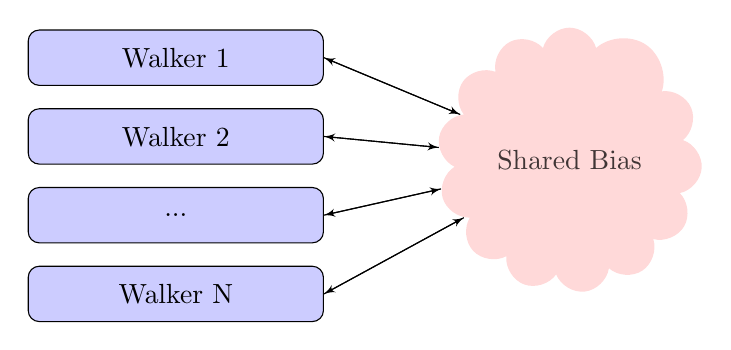
\begin{tikzpicture}[minimum size=5mm,node distance=4cm and 7cm,>=stealth,bend angle=45,auto]

         \node (Walker1) [block] {Walker 1};
         \node (Walker2) [block, below of=Walker1] {Walker 2};
         \node (points)  [block, below of=Walker2] {...};
         \node (WalkerN) [block, below of=points] {Walker N};

         \node (buffer) [cloud, cloud puffs=13.5, minimum width=3cm,minimum height=1.5cm, align=center, fill=red!20, opacity=0.75, right of=Walker1, xshift=1cm, yshift=-1.3cm] {Shared Bias};

         \path [line] (Walker1.east) -- (buffer);
         \path [line] (buffer) -- (Walker1.east);

         \path [line] (Walker2.east) -- (buffer);
         \path [line] (buffer) -- (Walker2.east);

         \path [line] (points.east) -- (buffer);
         \path [line] (buffer) -- (points.east);

         \path [line] (WalkerN.east) -- (buffer);
         \path [line] (buffer) -- (WalkerN.east);

     \end{tikzpicture}
   \end{figure}
\end{frame}

\section{Benchmark Calculations}
\begin{frame}{Benchmark Calculations}
 System: Torsion of Cl-F-ethane in vacuum (PBEh-3c/def2-msvp)
  \begin{figure}[H]
  \centering
  \includegraphics[width=0.5\textwidth]{bilder/talk/clfeth}
  \end{figure}
\end{frame}

\begin{frame}{Benchmark: ABF}
Ramp function:
\begin{equation}
R(N^k)=\left\{\begin{array}{ll} N^k/N_{full}, & N^{k} < N_{full} \\
                                             1, & N^{k} \geq  N_{full}\end{array}\right.
\end{equation}
  \begin{figure}[H]
      \centering
      \includegraphics[width=0.99\textwidth]{bilder/benchmark/ABF_benchmark_nfull}
      \caption{Influence of ramp function on convergence of ABF for torsion angle of Cl-F-ethane.}
  \end{figure}
\end{frame}

% \begin{frame}{Benchmark: eABF/CZAR}
%   Ramp function:
%   \begin{equation}
% R(N^k)=\left\{\begin{array}{ll} N^k/N_{full}, & N^{k} < N_{full} \\
%                                              1, & N^{k} \geq  N_{full}\end{array}\right.
% \end{equation}
%   \begin{figure}[H]
%       \centering
%       \includegraphics[width=0.99\textwidth]{bilder/benchmark/eABF_benchmark_ramp}
%       \caption{Influence of ramp function on convergence of eABF for torsion angle of Cl-F-ethane. $\sigma_\lambda = 5$ degree, $m_\lambda = 5$~a.u.}
%   \end{figure}
% \end{frame}

\begin{frame}{Benchmark: eABF/CZAR}
 \begin{figure}[H]
  \centering
    \includegraphics[width=0.99\textwidth]{bilder/benchmark/eABF_benchmark_mass}
   \caption{Influence of mass of fictitious particle on convergence of eABF. $\sigma_\lambda=5$~degree, $N_{full}=100$.}
\end{figure}
\end{frame}

\begin{frame}{Benchmark: eABF/CZAR}
  Force constant of extended system:
  \begin{equation}
    k_i = \frac{k_B T}{\sigma_i^2}=\frac{1}{\beta\sigma_i^2}
  \end{equation}
  Variance of collected force samples $\propto \sigma_i^{-2}$
  \begin{figure}[H]
    \centering
      \includegraphics[width=0.99\textwidth]{bilder/benchmark/eABF_benchmark_sigma}
     \caption{Influence of $\sigma$ on convergence of eABF with $m_\lambda=15$~a.u. and $N_{full}=100$.}
  \end{figure}
\end{frame}

\begin{frame}{Benchmark: WTM-eABF/CZAR}
  \begin{equation}
  U^{WTM}(\xi,t)={\color{red}{W}}\text{e}^{-\frac{U^{WTM}(\xi,t-\tau_G)}{k_B \Delta T}}\sum_{t'=\tau_G,2\tau_G,...}^{t'<t} \text{e}^{-\frac{1}{2\sigma_{G}^{2}} (\xi(\textbf{x}(t))-\xi(\textbf{x}(t')))^2 }
\end{equation}
\begin{figure}[H]d
  \centering
    \includegraphics[width=0.99\textwidth]{bilder/benchmark/meta_eABF_benchmark_height}
   \caption{Influence of Gaussian height on convergence of WTM-eABF with $m_\lambda=5$~a.u., $\sigma_\lambda=5^\circ$, $\sigma_G=5^\circ$, $\tau_G=10$~fs, $\Delta T=2000$~K and $N_{full}=100$.}
\end{figure}
\end{frame}

\begin{frame}{Benchmark: WTM-eABF/CZAR}
\begin{equation}
  U^{WTM}(\xi,t)=W\text{e}^{-\frac{U^{WTM}(\xi,t-\tau_G)}{k_B \Delta T}}\sum_{t'=\tau_G,2\tau_G,...}^{t'<t} \text{e}^{-\frac{1}{2{\color{red}{\sigma_{G}}}^{2}} (\xi(\textbf{x}(t))-\xi(\textbf{x}(t')))^2 }
\end{equation}
\begin{figure}[H]
  \centering
    \includegraphics[width=0.99\textwidth]{bilder/benchmark/meta_eABF_benchmark_var}
   \caption{Influence of Gaussian variance on convergence of WTM-eABF with $m_\lambda=5$~a.u., $\sigma_\lambda=5^\circ$, $W=5$~kJ/mol, $\tau_G=10$~fs, $\Delta T=2000$~K and $N_{full}=100$.}
\end{figure}
\end{frame}

\begin{frame}{Benchmark: Convergence acceleration}
\begin{figure}[H]
  \centering
    \includegraphics[width=0.99\textwidth]{bilder/benchmark/ABF_acc_benchmark}
   \caption{Top: Convergence of ABF, eABF and WTM-eABF. Blue: normal simulation, Orange: Shared bias with two walkers started from product and educt state, respectively, Green: Stratified to two windows of equal size.
  Bottom: Trajectories of normal ABF, eABF and WTM-eABF simulations}
\end{figure}
\end{frame}

\section{Application to Sirtuin 5}
\begin{frame}{Application to Sirtuin 5}
  \begin{itemize}
   \item System: Small toy model of the reactive center of Sirt5 (HF3c/minix in vacuum)
   \item Collective variable: $\xi=d_{CO}-d_{CN}$
   \item Enhanced Sampling: WTM-eABF with $\sigma_\lambda=0.5$~$\AA$, $m_\lambda=30$~a.u., $\sigma_G=0.1$~$\AA$, $W=2.0$~kJ/mol, $\tau_G=10$~fs and $\Delta T=4000$~K
   \item Free energy estimate: CZAR
\end{itemize}
\begin{figure}[H]
  \centering
    \includegraphics[width=0.5\textwidth]{bilder/talk/sirt52050}
    \caption{Transition state of the methylation reaction in Sirtuin 5.}
\end{figure}
\end{frame}

\begin{frame}{Application to S\textsubscript{n}2 reaction of Sirtuin 5}
   \begin{figure}[H]
     \centering
       \includegraphics[width=0.9\textwidth]{bilder/talk/sirt5_SW_bohr}
      \caption{Application of WTM-eABF to Sirt5.}
   \end{figure}
\end{frame}

\begin{frame}{Application to S\textsubscript{n}2 reaction of Sirtuin 5}
   \begin{figure}[H]
     \centering
       \includegraphics[width=0.90\textwidth]{bilder/talk/sirt5_US}
      \caption{PMF obtained from WTM-eABF compared to Umbrella Sampling (22x25~ps simulation time)}
   \end{figure}
\end{frame}

\begin{frame}
\begin{center}
\Huge Questions?
\end{center}
\end{frame}


\end{document}
